%\documentclass[12pt]{report}
\documentclass[12pt]{article}
\usepackage{blindtext}
\usepackage[T1]{fontenc}
\usepackage[utf8]{inputenc}
\usepackage{float}

\usepackage{amssymb}

\usepackage{amsmath}
\usepackage{graphicx}
\usepackage{amsthm}
\usepackage{multirow}
\usepackage{mathtools}
\usepackage{listings}
\usepackage{glossaries}


\newtheorem{definition}{Definition}
\DeclareMathOperator*{\argmax}{argmax} 
\DeclareMathOperator*{\argmin}{argmin} 
\DeclareMathOperator*{\max2}{max} 

\makeglossaries
\newglossaryentry{cnn}
{
	name=cnn,
	description={Convolutional neural network}
}

% Title Page
\title{Report on \textit{Evaluation and Design of Robust Neural Network Defenses}}
\author{Reporter: Duc-Anh Nguyen, PhD Student\\VNU Vietnam National University}

\date{}
\begin{document}
\maketitle

\newpage
\begin{center}
	\textbf{Disclaimer}
\end{center}
This work is done based on my understanding of the chosen author' publications in particular and the foundation of machine learning in general. Therefore, what I presented here may be incorrect to some extent. If readers have any comment on my report, please feel free to contact me. The comment of other readers are valuable to me.

I would like to thank Prof. Thuy Ha Quang, Prof. Thuan Ninh Truong, and Prof. Ha Viet Nguyen about their valuable knowledge about lectures about research methods and latex skills. This report is done on latex and available at.

\newpage
\begin{center}
	\textbf{About author}
\end{center}

Nicholas Carlini\footnote{https://nicholas.carlini.com} is a research scientist at Google Brain working at the intersection of machine learning and computer security. His most recent line of work studies properties of neural networks from an adversarial perspective. He received Ph.D. from UC Berkeley in 2018, and B.A. in computer science and mathematics (also from UC Berkeley) in 2013. 
Generally, he is interested in developing attacks on machine learning systems; most of his work develops attacks demonstrating security and privacy risks of these systems. He has received best paper awards at ICML and IEEE S\&P, and his work has been featured in the New York Times, the BBC, Nature Magazine, Science Magazine, Wired, and Popular Science. 
Previously he interned at Google Brain, evaluating the privacy of machine learning; Intel, evaluating Control-Flow Enforcement Technology (CET); and Matasano Security, doing security testing and designing an embedded security CTF.

From my perspective, both his research and my research interests are related to the topic "testing for AI systems". His academic background is really good. The chosen thesis is developed from the paper "Towards Evaluating the Robustness of Neural Networks" presented at IEEE S\&P in 2017. With this paper, he received the best student paper award.

I am really execited to read the research of Nicholas Carlini et al. to strengthen my research background in this topic. The expectation includes but not limited to (1) mathematics, (2) the way he organized the thesis to convince the council, and (3) dig into new idea behind this thesis.

%Summary the work of Nicholas Carlini\footnote{https://nicholas.carlini.com}: the key point, the structure of thesis

%Explain why  I choose his topic among other topics related to adversarial sample generation.

%The expectation after reading this thesis

%\begin{abstract}
%\end{abstract}

%\clearpage
%\textbf{Glossary}
%\printglossary[type=\acronymtype]

\newpage
\tableofcontents

\newpage

\listoffigures

\listoftables

\newpage
\section{Introduction}

Neural network has been used widely in solving many problems related to classification, ranging from speech processing \cite{speech-processing}, image processing \cite{image-processing}, to medical diagnosis \cite{medical-diagnosis}, etc. In most of the cases, if neural network models are trained with appropriate hyperparameters, the accuracy of these models usually outperform traditional machine learning teachniques such as Naive Bayes, K-nearest neighbors (KNN), etc. However, neural network models are usually unexplainable. Therefore, the testing of neural network models should be taken into account to ensure the correctness of these models.

Although the testing for neural network models is urgent and important, it has just been at the early stage from the research community and ML software companies \cite{DeepXplore}.  \textit{First}, to the best of my knowledge, to evaluate the reliability of neural network models for classification problem, most of ML researchers/developers usually make use of traditional criteria. Specifically, ML practitioners use precision, accuracy, F1-score, ROC, etc. to evaluate the quality of neural network models. However, these kinds of criteria just consider the input and output of neural network models without its internal structure. As a result, good results of traditional criteria do not mean that neural network models have no fault. Therefore, although traditional criteria seem to be effective to evaluate the reliability of neural network models, it is not enough. 
%In this case, white-box testing should be applied to check the correctness of neural network models. 
\textit{Second}, the testing phase of neural network models is usually performed manually by ML practitioners most of the time. These practitioners give a little concern about how to test neural network models automatically. Even if they spend more efforts on testing neural network models automatically, there are only a limited set of automated testing tools for neural network models up to now. 
%Hence, the testing of neural network models should be automated to reduce to cost of the testing phase.

To address the above problems, Nicholas Carlini et al. aimed to focus on testing the correctness of neural networks by attacking these models. The authors realized that neural network models, even these models are proved good enough, are prone to evasion attack. Evasion attack is a type of attack in which neural network models are fed with adversarial samples. In this context, evasion attack, known as \textit{adversarial samples}, can be described as follows: Given a sample $x$ (may be classified correctly or not by a neural network model) and a target class $t$, it is possible to find $x'$ which is classified as class $t$, and $x'$ is close to $x$. Term \textit{close} means that there is no significant differences between $x$ and $x'$ in terms of norm distance such as $||L||_0$, $||L||_1$, $||L||_2$, or $||L||_\infty$. 

From the given problem statement, the authors proposed three kinds of attacks, namely $||L||_2$ attack, $||L||_0$ attack, and $||L||_\infty$ attack. However, this report only focus on $||L||_2$ attack and $||L||_0$ attack which I understand the best and can spend more time on digging the implementation of these attacks. $||L||_2$ is highly recommended among the three proposed attacks. In order to evaluate the effectiveness of the proposed attacks, their experiment was performed on three type of applications including (i) breaking defenses of existing neural network models, (ii) speech recognition, and (iii) malware classification. The source code of the thesis is fully available here\footnote{https://github.com/carlini/nn\_robust\_attacks}.

This remaining part of this report includes 7 sections. Firstly, the report presents related works which are synthesised from the resources I have covered so far, including the thesis of the authors. After that, I describe the problem formulation which is summarized in the thesis. The next section provides the background about the related techniques/mathematics to adversarial samples. The report continues with dataset section giving the description about the dataset used in the experiment, and the result of rebuit model made by me. The proposed attacks section presents the attacks which the author suggested. Finally, the report concludes in the last section.

\section{Related Works}

Currently, some works have been proposed for testing neural network model by several
research groups. Focusing only on the most recent and closest ones, we can refer to \cite{DeepXplore}, \cite{deep-gauge}, \cite{deepct}, \cite{deeproad}, \cite{deeptest}, \cite{concolic-testing}, and \cite{coverage-limiation}.

Pei et al. proposed DeepXplore \cite{DeepXplore} which is known as the first white-box testing technique for \textit{deep neural network} (DNN) models. The authors introduced a new coverage criterion, namely neuron coverage, which is used to assert the correctness of DNN models. The authors also present a method to generate adversarial data set from the original training set to enrich the training set. %Fig.~\ref{fig:example_of_deepxplore} gives an example of erroneous behaviour found by DeepXplore. The right side is the adversarial sample generated from the original sample. The left side is the original sample used in the training process.

Ma et al. \cite{deep-gauge} claimed that many state-of-the-art AI systems suffer from vulnerabilities which may result in serve consequences when applied to real-world applications. The authors claimed that measuring the quality of deep learning systems in terms of traditional measurements (i.e., accuracy, precision, or F1 score) is not enough. Therefore, the authors proposed a set of coverage criteria to evaluate the correctness of DNN models at the unit level, the integration level, and the system level. The authors made a comparison between neuron coverage presented in DeepXplore \cite{DeepXplore} and their proposed criteria. As a result, the proposed criteria are better than neuron coverage.

Tian et al. proposed Deeptest \cite{deeptest} to test automatically the quality of DNN models used in autonomous cars. The authors aimed to find out erroneous behaviours of DNN-driven vehicles that can potentially lead to fatal crashes. In the experiment, DeepTest found thousands of erroneous behaviours under different realistic driving conditions (e.g., blurring, rain, fog, etc.).

Sun et al. \cite{concolic-testing} suggested the application of concolic testing in DNN models evaluation. The authors utilized neuron coverage, modified condition-decision coverage, and neuron boundary coverage to check the quality of DNN models.

Zhang et al. proposed DeepRoad \cite{deeproad} to automatically testing the consistency of DNN-based autonomous driving systems. DeepRoad tries to generate driving scenes under various weather conditions to enrich the training data. To do that, the authors apply Generative Adversarial Networks (GANs) \cite{gan}. The experiments have shown that DeepRoad can detect thousands of inconsistent behaviours to improve the robustness of ML systems.

Ma et al. proposed DeepCT \cite{deepct} to evaluate the robustness of deep learning systems. DeepCT stands for deep combinatorial testing. The authors also introduce a set of criteria for testing deep learning systems. With the proposed coverage criteria, DeepCT tests the interactions of input to reduce the size of the test suite rather than exploring all the possible combinations of input space.

Li et al. investigated the advantages and disadvantages of structural coverage criteria \cite{coverage-limiation}. The study has shown the inconsistency between the distribution of adversarial examples and the distribution of samples. Therefore, the current coverage criteria should be improved to reduce this inconsistency and increase the robustness of adversarial examples generation.

\section{Problem formulation}

The author started from the original formula of adversarial sample generations, proposed by Szegedy et. al. \cite{42503}, defined as follows:

Given a n-dimensional vector $x \in \mathbb{R}^n$ in which $x$ is classified incorrectly: $C(x) \ne t$, where $t$ is the true class of $x$. We need to find $x' = x + \delta \in \mathbb{R}^n$ such that $x'$ is valid and predicted correctly while $x'$ is close to $x$ as follows:

\begin{equation}
\begin{split}
\label{eqn:original-adversarial-sample-formula}
\text{minimize } D(x, x + \delta)
\\
\text{such that } x + \delta \in [0..1]^n
\\
\text{and } C(x+\delta) = t
\end{split}
\end{equation}

However, the formula (\ref{eqn:original-adversarial-sample-formula}) is hard to solve in practice due to the high level complexity of $C(x+\delta) = t$. In fact, $C(x+\delta) = t$ is highly non-linear which struggles to solve. Therefore, Szegedy et. al. suggested that formula (\ref{eqn:original-adversarial-sample-formula}) should be redefined to make it easier to solve.

Normally, formula (\ref{eqn:original-adversarial-sample-formula}) is that  $C(x+\delta) = t$ is removed while adding a new formula $f(x+\delta) <= 0$: $C(x+\delta) = t$ if and only if $f(x+\delta) <= 0$.

\begin{equation}
\begin{split}
\label{eqn:modified-adversarial-sample-formula-v1}
\text{minimize } D(x, x + \delta)
\\
\text{such that } f(x+\delta) <= 0 
\\
\text{and } x + \delta \in [0..1]^n
\end{split}
\end{equation}

In formula (\ref{eqn:modified-adversarial-sample-formula-v1}), we have many choices to the function $f$, for example, cross-entropy function.

Szegedy et. al.  used a similar approach by proposing that formula (\ref{eqn:modified-adversarial-sample-formula-v1}) is written in another way as follows:

\begin{equation}
\begin{split}
\label{eqn:modified-adversarial-sample-formula-v2}
\text{minimize } D(x, x + \delta) + c \cdot f(x+\delta)
\\
\text{such that } x + \delta \in [0..1]^n
\end{split}
\end{equation}
, where $c > 0$ is a constant and $f(x+\delta) <= 0$.

\section{Background}

This section provides background on adversarial samples generation mentioned in the original paper. Firstly, this report describes $||L||_p$ norm which is used to compute the distance between two k-dimensional vectors. After that, the detail description of standard gradient descent and its variants are presented. Finally, the report covers box-constraints technique used to generate valid images.

%\subsection{Neural network}
%
%\begin{definition}
%	\textbf{Feedforward neural network}. A feedforward neural network, or FNN, is a tuple $N = (L, W, \theta)$, where $L = \{L_k|k \in {0 .. K-1}\}$ is a set of layers (i.e., the input layer, hidden layers, and the output layer). $K$ is the number of layers. $W \subseteq \{L \times L\}$ is a set of weights between all pair of layers, in which a pair of layers includes two consecutive layers. $\theta = \{\theta_k|k \in {1..K}\}$ is a set of activations in which each activation belongs to a layer. Each layer $L_k$ has $s_k$ neurons.
%\end{definition}
%
%Given a sample $x$ and a FNN $N = (L, W, \theta)$, the prediction of this sample is one dimensional array, denoted by:\[\hat{y}(x)= \{N_0(x), N_1(x), .., N_{s_{K-1}}(x)\}\], where $N_i(x) \in (0, 1)$ is the prediction probability of $x$ in the class \textit{i}-th. The prediction label of sample $x$ is denoted by $c(\hat{y}(x))$:
%\[c(\hat{y}(x))= \argmax_{0<=c <=s_{K-1}} N_c(x)\]
%
%A deep neural network, denoted by DNN, is a FNN with more than 2 layers.
%
%Training a FNN model: optimizer, learning rate, hyperparameters, etc.
%
%\begin{definition}
%	\textbf{Neuron}. Neuron \textit{j}-th of a layer $L_i \in L$ in a feedforward neural network $N = (L, W, \theta)$, denoted by $n_i(j)$, is associated with an activation function $\theta_i \in \theta$. The input value and the out value of the neuron are denoted by $u(n_i(j))$ and $v(n_i(j))$, respectively. The input value $u(n_i(j)) $ is computed based on the linear combination of the weights and the associated bias: $u(n_i(j)) =  b_i(j) + \sum_{n=0}^{s_{i-1}} w_{i-1,i}(n,j)$. The output value $v(n_i(j))$ is computed as follows: $v(n_i(j)) = \theta_i(u(n_i(j)))$.
%\end{definition}
%
%\begin{definition}
%	\textbf{Activation function}. Given a feedforward neural network $N = (L, W, \theta)$, the activation function of a layer $L_k$ (k>=0), denoted by $\theta_k$, is linear (e.g., identity, etc.) or non-linear (e.g., tanh, ReLU, sigmoid, softmax, etc.).
%\end{definition}
%
%Identity function of the neuron $n_i(j)$ is defined as follows:
%\[
%u(n_j(j)) = v(n_i(j))
%\]
%
%ReLU function of the neuron$n_i(j)$ is a commonly used activation function \cite{deepfault} \cite{DeepXplore} and defined as follows:
%\[
%v(n_i(j)) = \begin{dcases}
%u(n_i(j)) & when\hspace{0.1cm} u(n_i(j)) >= 0\\
%0 & otherwise
%\end{dcases}
%\]
%
%Softmax function of the neuron $n_i(j)$ is defined as follows:
%\[
%v(n_i(j)) = \frac{e^{u_i(j)}}{\sum_{k=0}^{s_i}{e^{u_i(j)}}} \in (0..1)
%\]
%
%Sigmoid function is a special case of softmax funtion when $s_i$ = 2.
%
%Tanh function of the neuron $n_i(j)$ is defined as follows:
%\[
%v(n_i(j)) = \frac{e^{u_i(j)} - e^{-u_i(j)}}{e^{u_i(j)} + e^{-u_i(j)}} \in (-1..1)
%\]

\subsection{$||L||_p$ norm}

Let $D(x, x') \in [0, \infty]$ be the distance between sample $x \in \mathbb{R}^n$ and $x' \in \mathbb{R}^n$ in which $x'$ is an adversarial example of $x$. $D(x, x') = 0$ if and only if both $x$ and $x'$ are identical.

The are many ways to calculate the distance between $x$ and $x'$, known as $ ||L_p||$ norm. The popular types of distance caculation are $L_0$ (p=0), $L_2$ (p=2), and $L_\infty$ (p=$\infty$).

The formula of $||L_p||$ is defined as follows:

\begin{center}
	$||L_p|| = (\sum_{i=0}^{n-1} (x_i-x'_i)^p)^{1/p} $
\end{center}

$||L_0||$ distance is interpreted as the number of different pixels when comparing between $x$ and $x'$.

$||L_2||$ distance is known as Euclidean distance. One major weakness of $||L_2||$ distance is that it may be a small value even when there are many changes in value of pixels between $x$ and $x'$.

$||L_\infty||$ distance measure the maximum change in value of pixels in every axis of the coordinate. Goodfellow et al. claimed that this metric is optimal to use in adversarial sample generation \cite{DBLP:journals/corr/GrossePM0M16}.

\begin{center}
	$||L_\infty|| = max(|x_0 - x'_0|, |x_1 - x'_1|, .., |x_{n-1} - x'_{n-1}|)$ 
\end{center}

\subsection{Gradient Descent}

Given the objective function $f(x)$, find $x$ to minimize $f(x)$. Gradient descent is a effective technique to seek for the $x$. This section covers standard gradient descent and its variants known as \textit{momentum gradient descent} and \textit{nesterov acclerated gradient}.

\subsubsection{Standard gradient descent}
	
The main idea of \textit{standard gradient descent }is that $x$ is modified iteratively in the opposite direction of $f'(x)$. The formula of the standard gradient descent can be written as follows:

\begin{equation}
	\label{eqn:sgd}
	x_{i+1} = x_{i} - \eta * f'(x) (i >= 0)
\end{equation}
, where $\eta$ is learning rate, $x$ is a $k$-dimensional vector, $x_0 = x$.

In formula (\ref{eqn:sgd}), learning rate $\eta$ is a hyperparameter and should be fine-tuned. There are several main points about the formula (\ref{eqn:sgd}).

\begin{itemize}
	\item Initialize $\eta$.  Usually, $\eta$ is initialized at a relatively small positive value, e.g., $\eta = 0.01$ or $\eta = 0.001$. If the value of $\eta$ is too small, the process of gradient descent may take larger number of iterations, leading to a waste of time. Otherwises, in the case that the value of $\eta$ is large, gradient descent process may go over the optimal value of $x$ due to the large jump of $x$.
	\item Constant $\eta$. Depending on the type of gradient descent technique, the value of learning rate $\eta$ is a constant (e.g., standard gradient descent, Nesterov momentum) or can be changed during gradient descent process (e.g., step decay, exponential decay, $1/t$ decay).
	\item Sign of $f'(x)$ . There are two cases happening with the sign of $f'(x)$:
	
	\begin{itemize}
		\item If the value of derivative function $f'(x)$ is positive, $f'(x)$ is going up. In this case, in order to minimize $f(x)$, the value of $x$ should be reduced by a small amount.
		
		\item If the value of derivative function $f'(x)$ is negative, $f'(x)$ is going down. In this case, in order to minimize $f(x)$, the value of $x$ should increase further.
	\end{itemize}
\end{itemize}

\subsubsection{Momentum gradient descent}

Momentum gradient descent improves standard gradient descent by converging to the optimal $x$ faster. 

\begin{equation}
\begin{split}
\label{eqn:sgd-momentum}
v_{t} = \mu * v_{t-1} + \eta * f'(x)
\\
x = x - v_t
\end{split}
\end{equation}
, where $\eta$ is learning rate, $x$ is a $k$-dimensional vector.

Equivalently, the formula (\ref{eqn:sgd-momentum}) can be written as follows:
\begin{equation}
\begin{split}
\label{eqn:sgd-momentum-v2}
x = x - (\mu * v_{t-1} + \eta * f'(x))
\end{split}
\end{equation}

Comparing to formula (\ref{eqn:sgd}), formula (\ref{eqn:sgd-momentum-v2}) adds $\mu * v_{t-1} $ representing the previous change of $x$, called \textit{momentum}. Momentum $\mu * v_{t-1} $ is accumulated over iterations.

\subsubsection{Nesterov accelerated gradient}

Nesterov accelerated gradient (NAG) improves momentum gradient descent by converging to the optimal $x$ faster. In order to do that, NAG will look ahead one iteration.

\begin{equation}
\begin{split}
\label{eqn:nag}
v_{t} = \mu * v_{t-1} + \eta * f'(x - \mu * v_{t-1})
\\
x = x - v_t
\end{split}
\end{equation}

Equivalently, the formula (\ref{eqn:nag}) can be written as follows:
\begin{equation}
\begin{split}
\label{eqn:sgd-momentum-v2}
x = x - (\mu * v_{t-1} + \eta * f'(x - \mu * v_{t-1}))
\end{split}
\end{equation}

\subsection{Box Constraints}

The essense of adversarial sample generations is that the original sample $x$ is modified into $x' = x + \delta$. This modification may lead to an invalid sample $x'$. Therefore, we need to align $x'$ to the available range of value. In this thesis, the available range of each pixel is in $[0..1]$.

The author investigated there method to deal with this problem:

\begin{itemize}
	\item \textit{Projected gradient descent}. At each step of the standard gradient descent, all the pixels out of available range is cut off. 
	
	This strategy has a limit: The cut-off pixel is the input of the next step in standard gradient descent, the result of adversarial sample generation may be affected.
	
	\item \textit{Clipped gradient descent}. Rather than performing the normalization of pixel value at each step of SGD, the clipping step is put into funtion $f(x+\delta)$. Specifically, they replace $f(x+\delta)$ with $f(min(max(x+\delta, 0), 1))$.
	
	
	\item \textit{Changes of variables}. Instead of using variable $\delta$, they use a new variable $w$ as follows:
	\begin{equation}
		\delta = 1/2 * (tanh(w) + 1) - x \label{eqn:change-of-variables}
	\end{equation},
	where $w, \delta, x$ is a n-dimensional vector.
	
	Because $tanh(w) \in [-1, 1]^n$, $1/2 * (tanh(w) + 1) \in [0, 1]^n$; hence $x + \delta \in [0,1]^n$. This formula (\ref{eqa:change-of-variables}) ensures that $x'$ is a valid image. 
\end{itemize}

\begin{definition}
	Objective function
\end{definition}


\section{Dataset}

The authors used the two primary datasets: MNIST, CIFAR to evaluate their proposed attacks. In this report, I just use dataset MNIST to reevaluate their experiments. I re-run the training process of MNIST dataset and report the results below.

\subsection{MNIST}
MNIST is a dataset of digit recognizer which can be found officially on Kaggle\footnote{https://www.kaggle.com/c/digit-recognizer/data}. The training set contains 60,000 samples. The test set has 10,000 samples.  Each sample on the dataset is an image with 28 pixel in width and 28 pixel in height. The value of each pixel is in range of 0 and 255, which indicates the lightness or darkness of that pixel.

%In the above experiment, value of every pixel in each image is scale in range of [0..1] first, then scale to [-0.5, 0.5].

\subsection{CNN model}
Table \ref{tab:CNN-architecture-MNIST} illustrates the configuration of \gls{cnn} model used to train MNIST. Figure \ref{fig:MNIST-implementation} described the corresponding implementation of this model in python. For example, starting with the input having shape \textit{(size of batch, height = 28, width = 28, n\_channel = 1)}, this input is passed through a convolution layer with kernel \textit{(3 x 3)}, 32 filters, and \textit{valid} padding. A convolution layer with \textit{valid padding} option ensure that the kernel of convolution layer only move in the input (i.e., not go out of the border). Therefore, the output of convolution layer with this padding has:
\begin{center}
	$width\_output = width\_input - width\_kernel + 1 = 28 - 3 + 1 = 26$, and
	
	$height\_output = height\_input - height\_kernel + 1  = 28 - 3 + 1 = 26$
\end{center}

Therefore, the output of the first convolutional layer has shape (width = 26, height = 26, n\_filters = 32).


% Please add the following required packages to your document preamble:
% \usepackage{graphicx}
\begin{table}[H]
	\centering
	\small
	\caption{CNN architecture of MNIST}
	\vspace{6mm}
	\label{tab:CNN-architecture-MNIST}
	%\resizebox{\textwidth}{!}{%
	\begin{tabular}{|l|l|}
		\hline
		\textbf{Layer Type} & \textbf{MNIST} \\ \hline
		Convolution + ReLU activation & kernel (3x3), 32 filters \\ \hline
		Convolution + ReLU activation & kernel (3x3), 32 filters \\ \hline
		Max Pooling & kernel (2x2) \\ \hline
		Convolution + ReLU activation & kernel (3x3), 64 filters \\ \hline
		Convolution + ReLU activation & kernel (3x3), 64 filters \\ \hline
		Max Pooling & kernel (2x2) \\ \hline
		Fully Connected + ReLU activation & 200 \\ \hline
		Fully Connected + ReLU activation & 200 \\ \hline
		Softmax & 10 \\ \hline
	\end{tabular}%
	%	}
\end{table}

\begin{figure}[H]
	\centering
	\caption{The implementation of CNN architecture used to train MNIST}
	\label{fig:MNIST-implementation}
	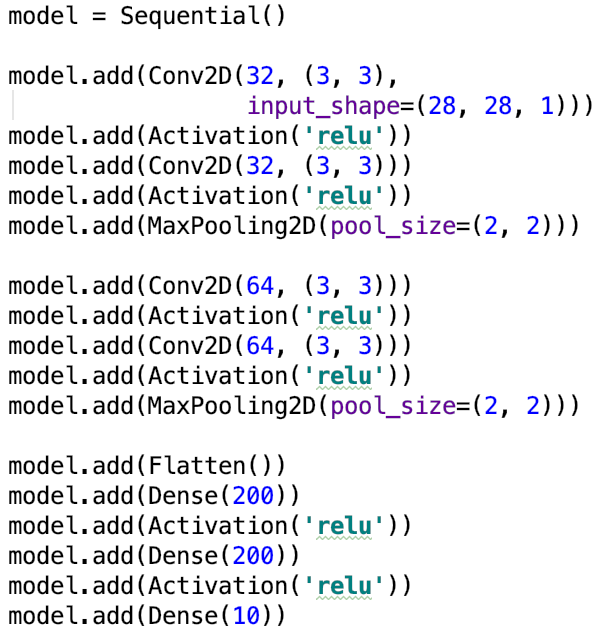
\includegraphics[scale=0.7]{img/MNIST}
	%\vspace{-4mm}	
\end{figure}


\subsection{Training}
The model is trained with the following fine-tuning hypeparameters: learning rate $\eta = 0.01$, decay = 1e-6, momentum = 0.9. To overcome optimal solution during batch gradient descent, they applied Nesterov momentum. The training process is taken in 50 iterations with batch = 128 samples. Like the orginal experiment, there is no data-set augmentation in the re-evaluation.

The achieved accuracy of CNN model is 0.9985\%. While figure \ref{fig:MNIST-accuracy} shows the accuracy over iterations when training MNIST, figure \ref{fig:MNIST-loss} illustrates the value of loss function over 50 iterations.

\begin{figure}[H]
	\centering
	\caption{Accuracy over iterations when training MNIST}
		\label{fig:MNIST-accuracy}
	\vspace{2mm}
	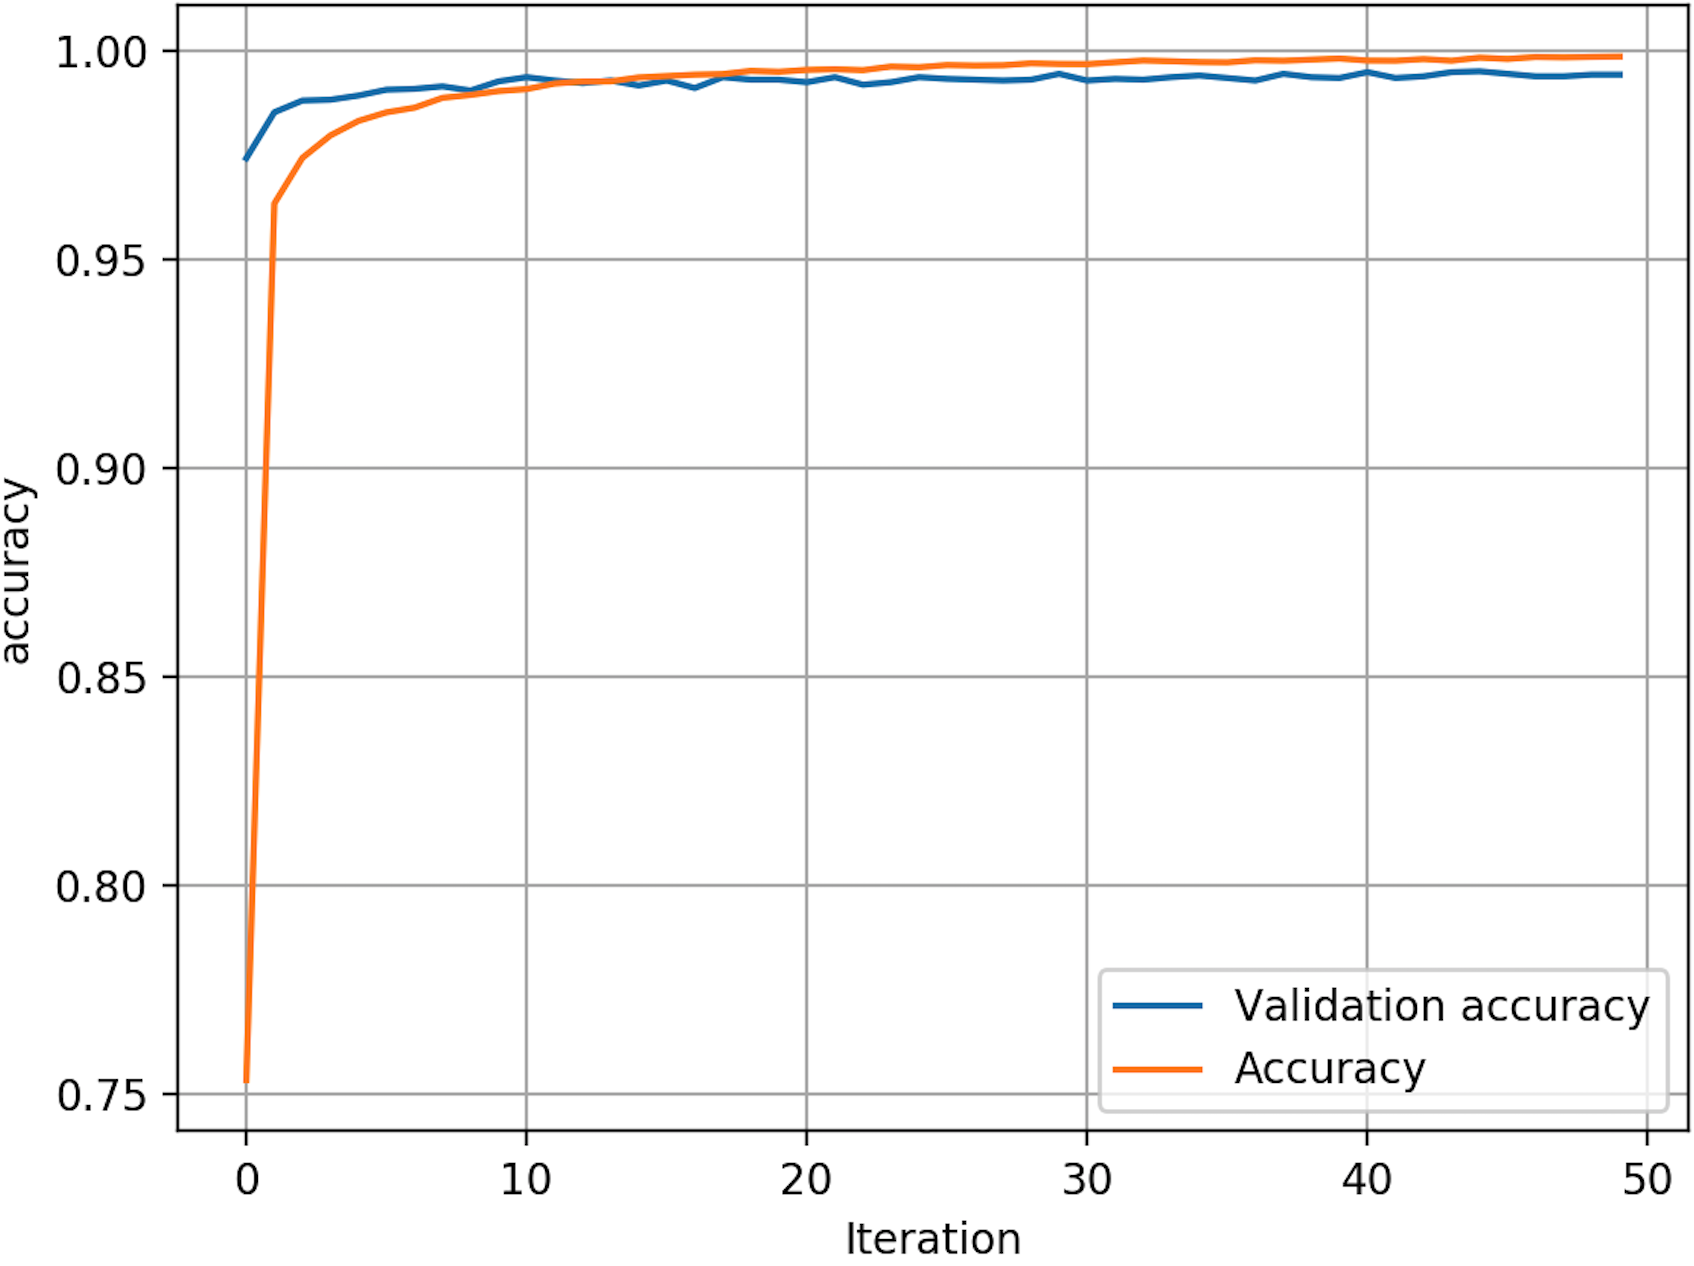
\includegraphics[scale=0.35]{img/MNIST_accuracy}
\end{figure}

\begin{figure}[H]
	\centering
	\caption{Loss over iterations when training MNIST}
		\label{fig:MNIST-loss}
	\vspace{2mm}
	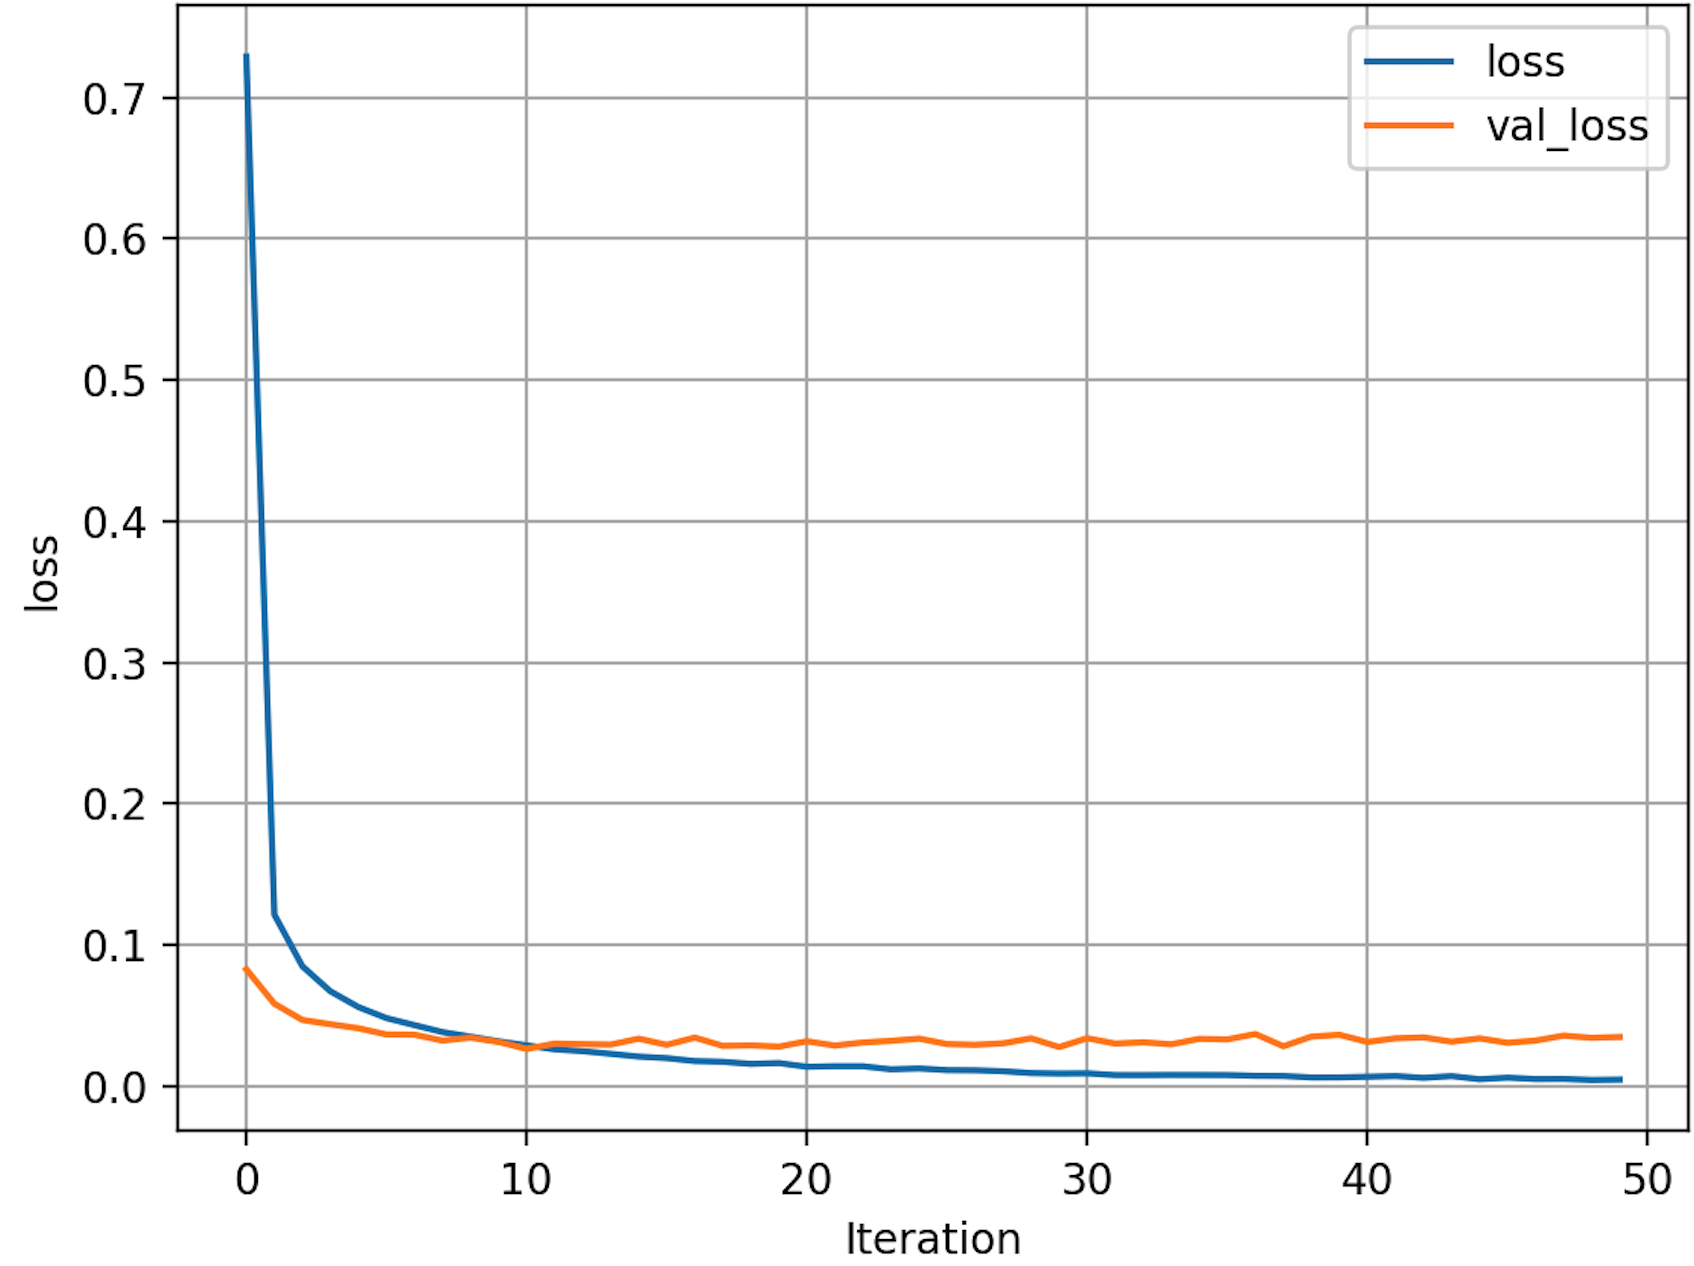
\includegraphics[scale=0.35]{img/MNIST_loss}
\end{figure}


\section{The proposed attacks}

The problem statement is as follows:

\begin{equation}
\begin{split}
\label{eqn:modified-adversarial-sample-formula-v2}
\text{minimize } D(x, x + \delta) + c \cdot f(x+\delta)
\\
\text{such that } x + \delta \in [0..1]^n
\end{split}
\end{equation}
, where $c > 0$ is a constant, $f(x+\delta) <= 0$, $x$ is the original sample, $x + \delta$ is a adversarial sample; $\delta$ is the difference between $x$ and $x'$, $D$ is norm distance.

For simplicity, the problem statement is rewritten as follows:

\begin{equation}
\begin{split}
\label{eqn:modified-adversarial-sample-formula-v6}
\text{minimize } ||\delta||_p + c \cdot f(x+\delta)
\\
\text{such that } x + \delta \in [0..1]^n
\end{split}
\end{equation}

In the above objective function (\ref{eqn:modified-adversarial-sample-formula-v6}), there are many formula of function $f(x+\delta)$ which have been proposed by many different research groups. In these formula, $f_1(x')$ is the most popular function $f$, which is known as cross-entropy function.

\begin{figure*}[h]
	\centering
	\vspace{-6mm}
	\vspace*{5mm} 
	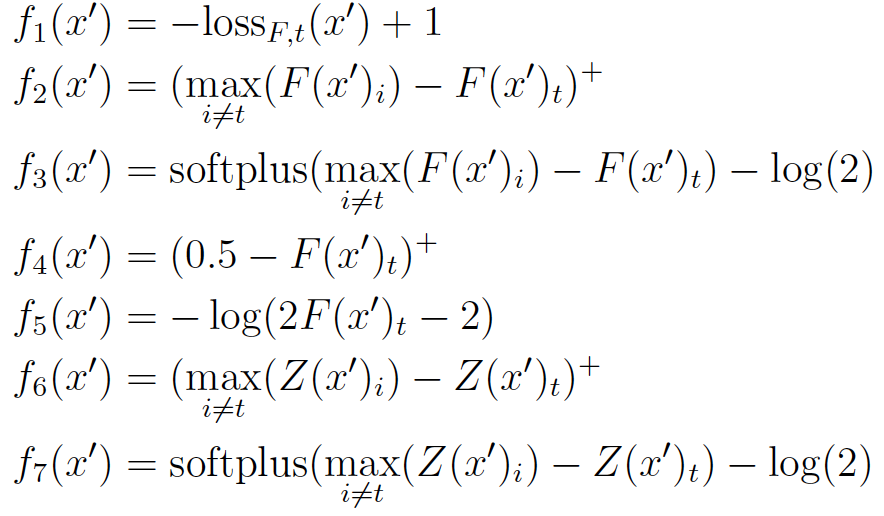
\includegraphics[scale=0.6]{img/f}
	\vspace{-4mm}	
\end{figure*}
, where $s$ is the correct classification; ($e)_+$ is short-hand for $max(e, 0)$; $softplus(x) = log(1+exp(x))$.

The authors took expriments to find the best function among $f_1(x')$ to $f_6(x')$. They conclude $f_6(x')$ showed the most significant result compared to the other functions.

Hence, the problem statement is refined as follows:

\begin{equation}
\begin{split}
\label{eqn:modified-adversarial-sample-formula-v6}
\text{minimize } ||\delta||_p + c \cdot max(\max2_{i \neq t} (Z(x')_i) - Z(x')_t), 0)
\\
\text{such that } x + \delta \in [0..1]^n
\end{split}
\end{equation}

The authors made use of "change of variable" method (formula \ref{eqn:change-of-variables}) which replaces $x + \delta$ with $w$.

\begin{center}
	\begin{equation}
	\begin{split}
	\label{eqn:modified-adversarial-sample-formula-v7}
	\text{minimize } ||1/2 * (tanh(w) + 1) - x||_p + 
	\\
	c \cdot max(\max2_{i \neq t} (Z(1/2 * (tanh(w) + 1) )_i) - Z(1/2 * (tanh(w) + 1) )_t), 0)
	\\
	\text{such that } 1/2 * (tanh(w) + 1)  \in [0..1]^n
	\end{split}
	\end{equation}
\end{center}

\subsection{$||L||_2$ attack}

Given the formula (\ref{eqn:modified-adversarial-sample-formula-v7}), the author tried to  generate adversarial samples. The original idea of  $||L||_2$ attack is as follows:

\begin{itemize}
	\item \textit{Step 0}. Start with target class $t$, the original sample $x$, and the neural network model $N$ trained before; $C^*(x) $ is the true class of $x$; $C(x) \ne t$ is the predicted class of $x$ given model $N$.
	
	\item \textit{Step 1}. Calculate the derivative of the objective function (\ref{eqn:modified-adversarial-sample-formula-v7}) with respect to $w$. Denote the objective function  as $G$, we need to compute $G'(w)$.
	
	\item \textit{Step 2}. Use standard gradient descent to compute $x_{i+1} = x_i - \eta * G'(w)$ iteratively, where constant $\eta$ is learning rate. At each iteration, compute the prediction of $x_{i+1}$. If $C(x_{i+1}) = t$, the algorithm terminates and report on $x_{i+1}$, denoted by $x'$.
	
	
\end{itemize}

The above $||L||_2$ attack has a major disadvantage. The returned $x'$ may be a local optimal solution which is caused by the chosen learning rate $\eta$. Since the research just used standard gradient descent, choosing small value of $\eta$ is just enough though it may take more iterations.

Instead of changing $\eta$, the authors proposed \textit{multiple starting-point gradient descent}. The idea of this technique is that rather than starting at $x$, $||L||_2$ attack starts with $x^* $ where $x^*$ is close to $x$. To reduce the cost of adversarial sample generation, the number of iterations in standard gradient descent is fixed since there are many similar point $x^*$.

% They randomly sample points uniformly from the ball of radius $r$, where $r$ is the closest adversarial example found so far. Intially, $r = 0$


An example of $||L||_2$ attack on MNIST is shown in Fig.~\ref{fig:L2-attack-sample}. The result of adversarial sample generation for s digit include three parts: (i) a source digit, (ii) target digit, and (iii) an adversarial image. Almost all attacks are visually indistinguishable from the original digit.

\begin{figure}[h]
	\centering
	\caption{Perform $||L||_2$ attack on MNIST}
		\label{fig:L2-attack-sample}
	%\vspace{-6mm}
	%	\vspace*{5mm} 
	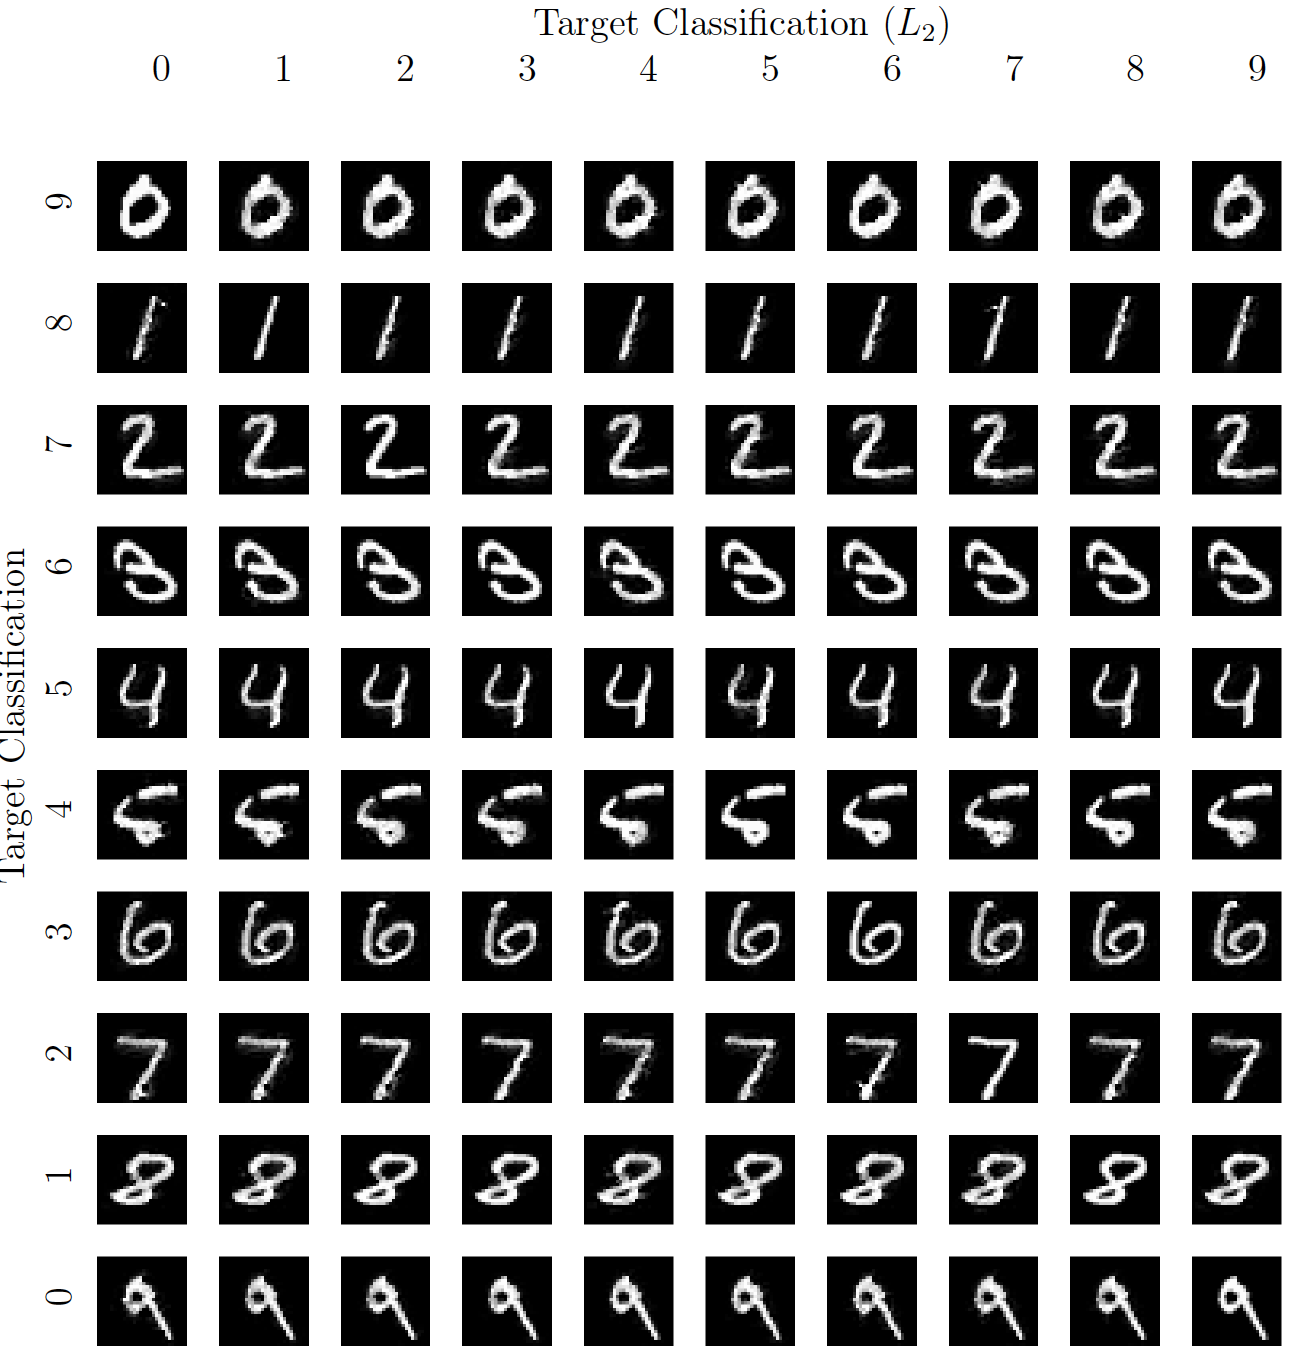
\includegraphics[scale=0.47]{img/L2-attack-sample}
	%	\vspace{-4mm}	
\end{figure}

\subsection{$||L||_0$ attack}
Because $||L||_0$ is non-differentiable, therefore, the authors proposed an interative algorithm to perform $||L||_0$ attack.

Rather than computing the derivative of both terms in formula (\ref{eqn:modified-adversarial-sample-formula-v7}, they just considered the second terms. The first term $||L||_0$ is ignored.

\begin{itemize}
	\item \textit{Step 0}. Start with target class $t$, the original sample $x$, and the neural network model $N$ trained before; $C^*(x) $ is the true class of $x$; $C(x) \ne t$ is the predicted class of $x$ given model $N$. Denote the allowed set $S$ containing all pixels in $x$. All the pixels out of $S$ are fixed (can not be changed). $S$ only contains the pixels which can be changed to generate adversarial samples $x'$.
	
	\item \textit{Step 1. Shrink the allowed set $S$}. 	Perform $||L||_2$ attack above with respect to the pixels in $S$. There are two cases happening:
	\begin{itemize}
		\item Case 1: Can not find adversarial sample. In this case, the algorithm terminates.
		\item Case 2: Find an adversarial sample $x_{i+1}$. Remove the pixel \textit{j}-th in $S$ which has the least influence on creating adversarial sample $x'$
		
		\begin{equation}
		j = \argmin_{j \in S} (f_6'(x_{i+1})_j * (x_{i+1} - x)_j)
		\end{equation}
		, where $(f_6'(x_{i+1})_j * (x_{i+1} - x)_j)$ tell us how much the reduction to $f_6'(x_{i+1})$ when moving $x$ to $x_{i+1}$; $f_6'(x_{i+1})$ is a 1-D vector when computing the value of $f'_6(x)$ at adversarial sample $x_{i+1}$; pixel \textit{j}-th in $S$ has the change per unit $f_6'(x_{i+1})_j$. 
		
		For the pixel \textit{j}-th having the least reduction, they removed it from $S$. They argued that this pixel does not have much influence on classifier output.
		
		Then repeat step 1.
	\end{itemize}
	
\end{itemize}

When performing $||L||_0$ attack, the value of constant $c$ is initialized to a very low value (e.g., $10^{-4}$). The threshold of $c$ should be high ()e.g., $10^{10}]$). At step 1, if $||L||_2$ attack can not found any adversarial sample, the value of $c$ is double until it reaches the limitation.

An example of $||L||_0$ attack on MNIST is shown in Fig.~\ref{fig:L0-attack-sample}.
The attacks are east to realize the diference because the $||L||_0$ attack is more difficult than $||L||_2$.

\begin{figure}[H]
	\centering
	\label{fig:L0-attack-sample}
	\caption{Perform $||L||_0$ attack on MNIST}
	%\vspace{-6mm}
%	\vspace*{5mm} 
	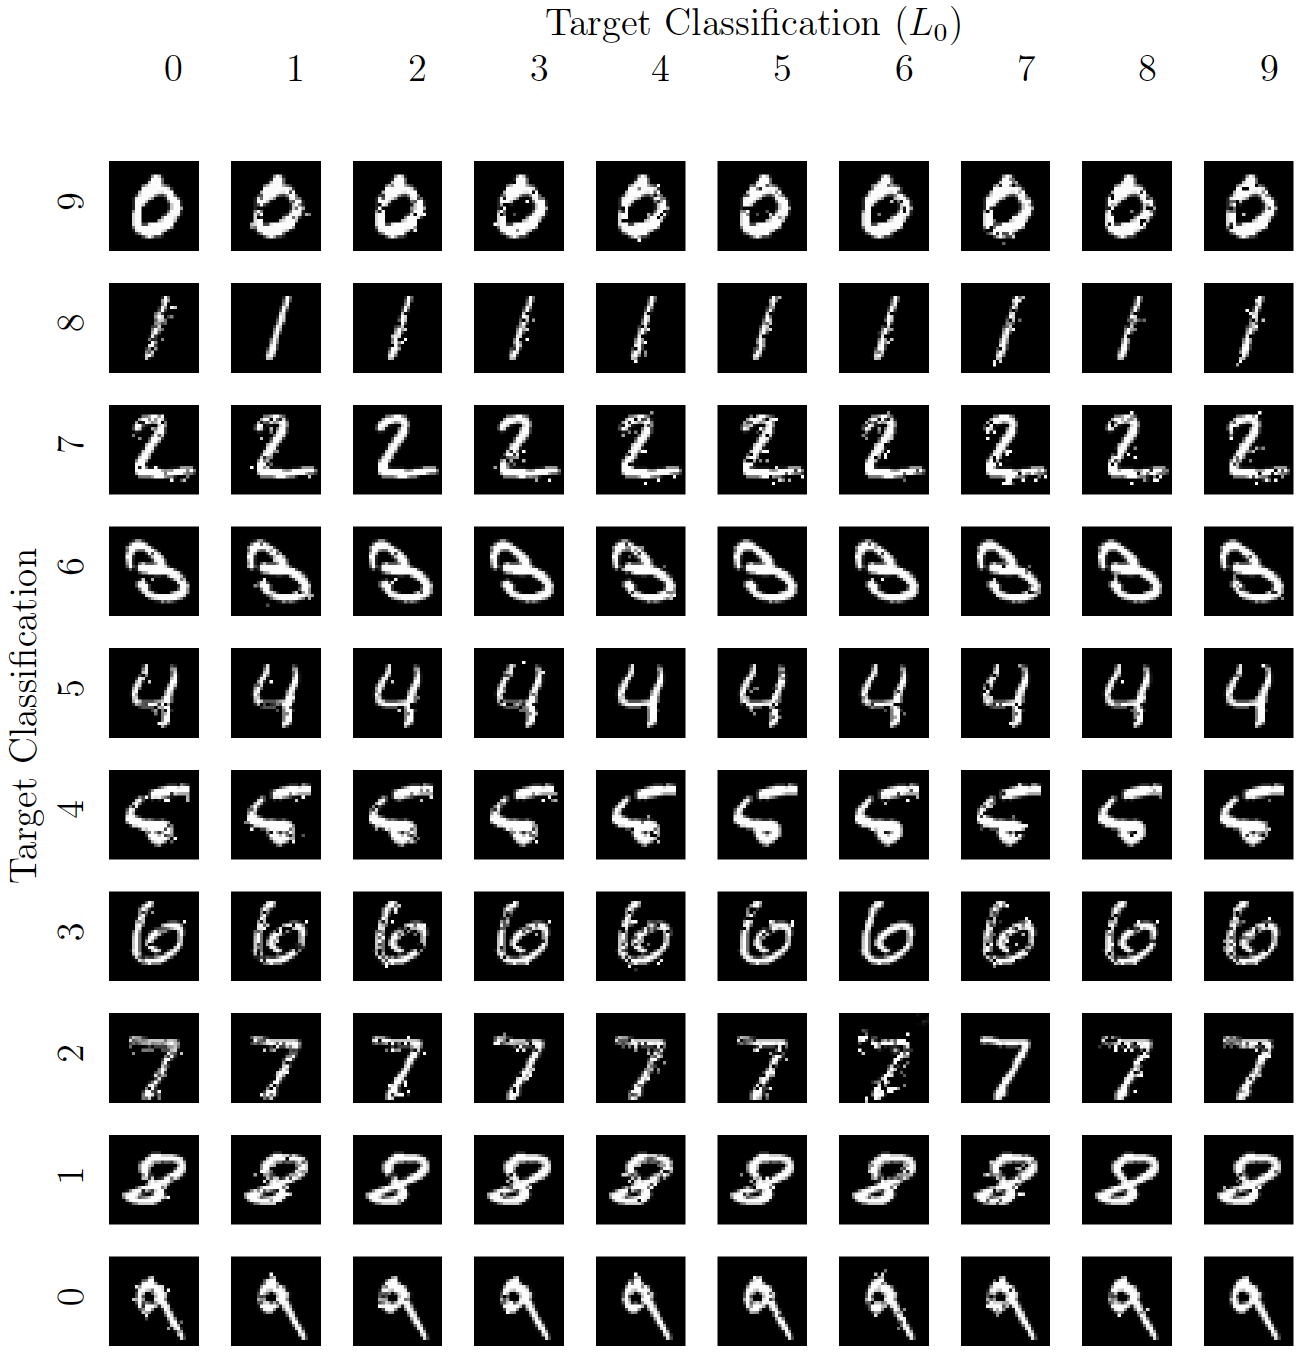
\includegraphics[scale=0.47]{img/L0-attack-sample}
%	\vspace{-4mm}	
\end{figure}

%\subsection{$||L||_\infty$ attack}
%
%\begin{figure}[H]
%	\centering
%	\label{fig:Linf-attack-sample}
%	\caption{Perform $||L||_\infty$ attack on MNIST}
%	%\vspace{-6mm}
%	%	\vspace*{5mm} 
%	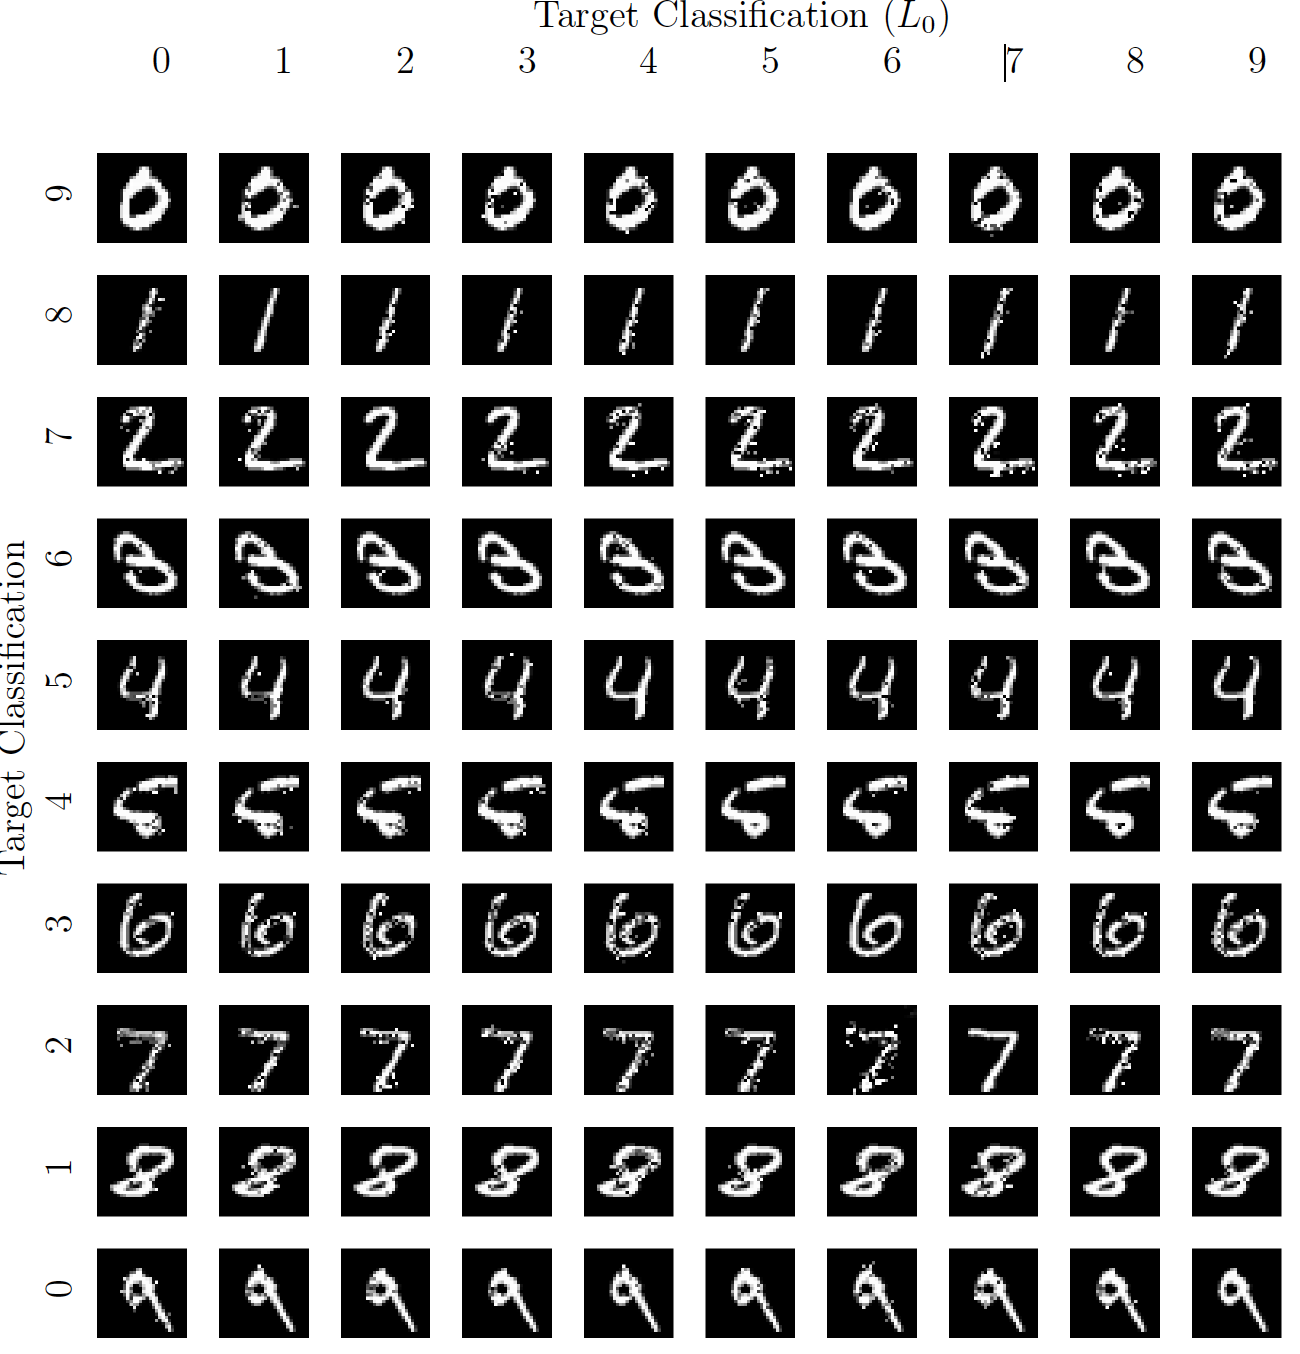
\includegraphics[scale=0.6]{img/Linf-attack-sample}
%	%	\vspace{-4mm}	
%\end{figure}
%
%An example of $||L||_\infty$ attack on MNIST is shown in Fig.~\ref{fig:Linf-attack-sample}.


\section{Conclusion}

The report covers the two efficient adversarial attacks: $||L||_0$ attack and $||L||_2$ attack. These types of attack aim to generate new sample from original samples in dataset which make wrong prediction. $||L||_0$ attack is an iterative algorithm which includes $||L||_2$ attack. The author stated that $||L||_2$ attack is better than $||L||_0$ attack via the expriment. Given an original sample and a target,  $||L||_2$ attack generate an adversarial sample which is closer to the original sample than $||L||_0$ attack. 

In order to have a better understanding about their proposals, I re-evaluate their experiments and dig deep into their source code. This thesis enriched my background about adversarial example generation in particular and machine learning in general. I am planning to take the following steps: (i) evaluate the quality of generated adversarial samples by using the current criteria such as neuron coverage \cite{DeepXplore}, kmnc/sbc/snac/tknc coverage \cite{deep-gauge}. I am implementing this kinds of criteria and push to my repository on github\footnote{https://github.com/ducanhnguyen/mydeepconcolic}. After evaluating the disadvantage and disadvantage of their proposed attacks, I will analyze the problem to improve these attacks.


\bibliography{bibitex_thesis} 
\bibliographystyle{ieeetr}

\end{document}          
